\documentclass[12pt]{article}

\usepackage{geometry, subfiles}
\usepackage{amsmath, amssymb}
\usepackage{booktabs, longtable, siunitx}
\usepackage{graphicx}
\graphicspath{{/Users/wonjun/Dropbox/Emory/ECON771_health2/assignments/assignment1/output/}}

\title{Assignment 1}
\author{Wonjun Choi}

\begin{document}
\maketitle
	\begin{itemize}
		\item[1.] Provide and discuss a table of simple summary statistics showing the mean, standard deviation, min, and max of hospital total revenues and uncompensated care over time.
		
		The summary statistics of hospital total revenues and uncompensated care over time are presented in Table 1 and 2, respectively. All of the statistics are scaled by million dollar. The tables show that both revenue and uncompensated care are increasing.
		\subfile{../output/tab_sumstat_rev}
		\subfile{../output/tab_sumstat_uncompcare}
		
		
		
		\item[2.] Create a figure showing the mean hospital uncompensated care from 2003 to 2019. Show this trend separately by hospital ownership type (private not for profit and private for profit).
		
		The mean hospital uncompensated care from 2003 to 2019 are shown in Figure 1.
		\begin{figure} [ht]
			\centering
			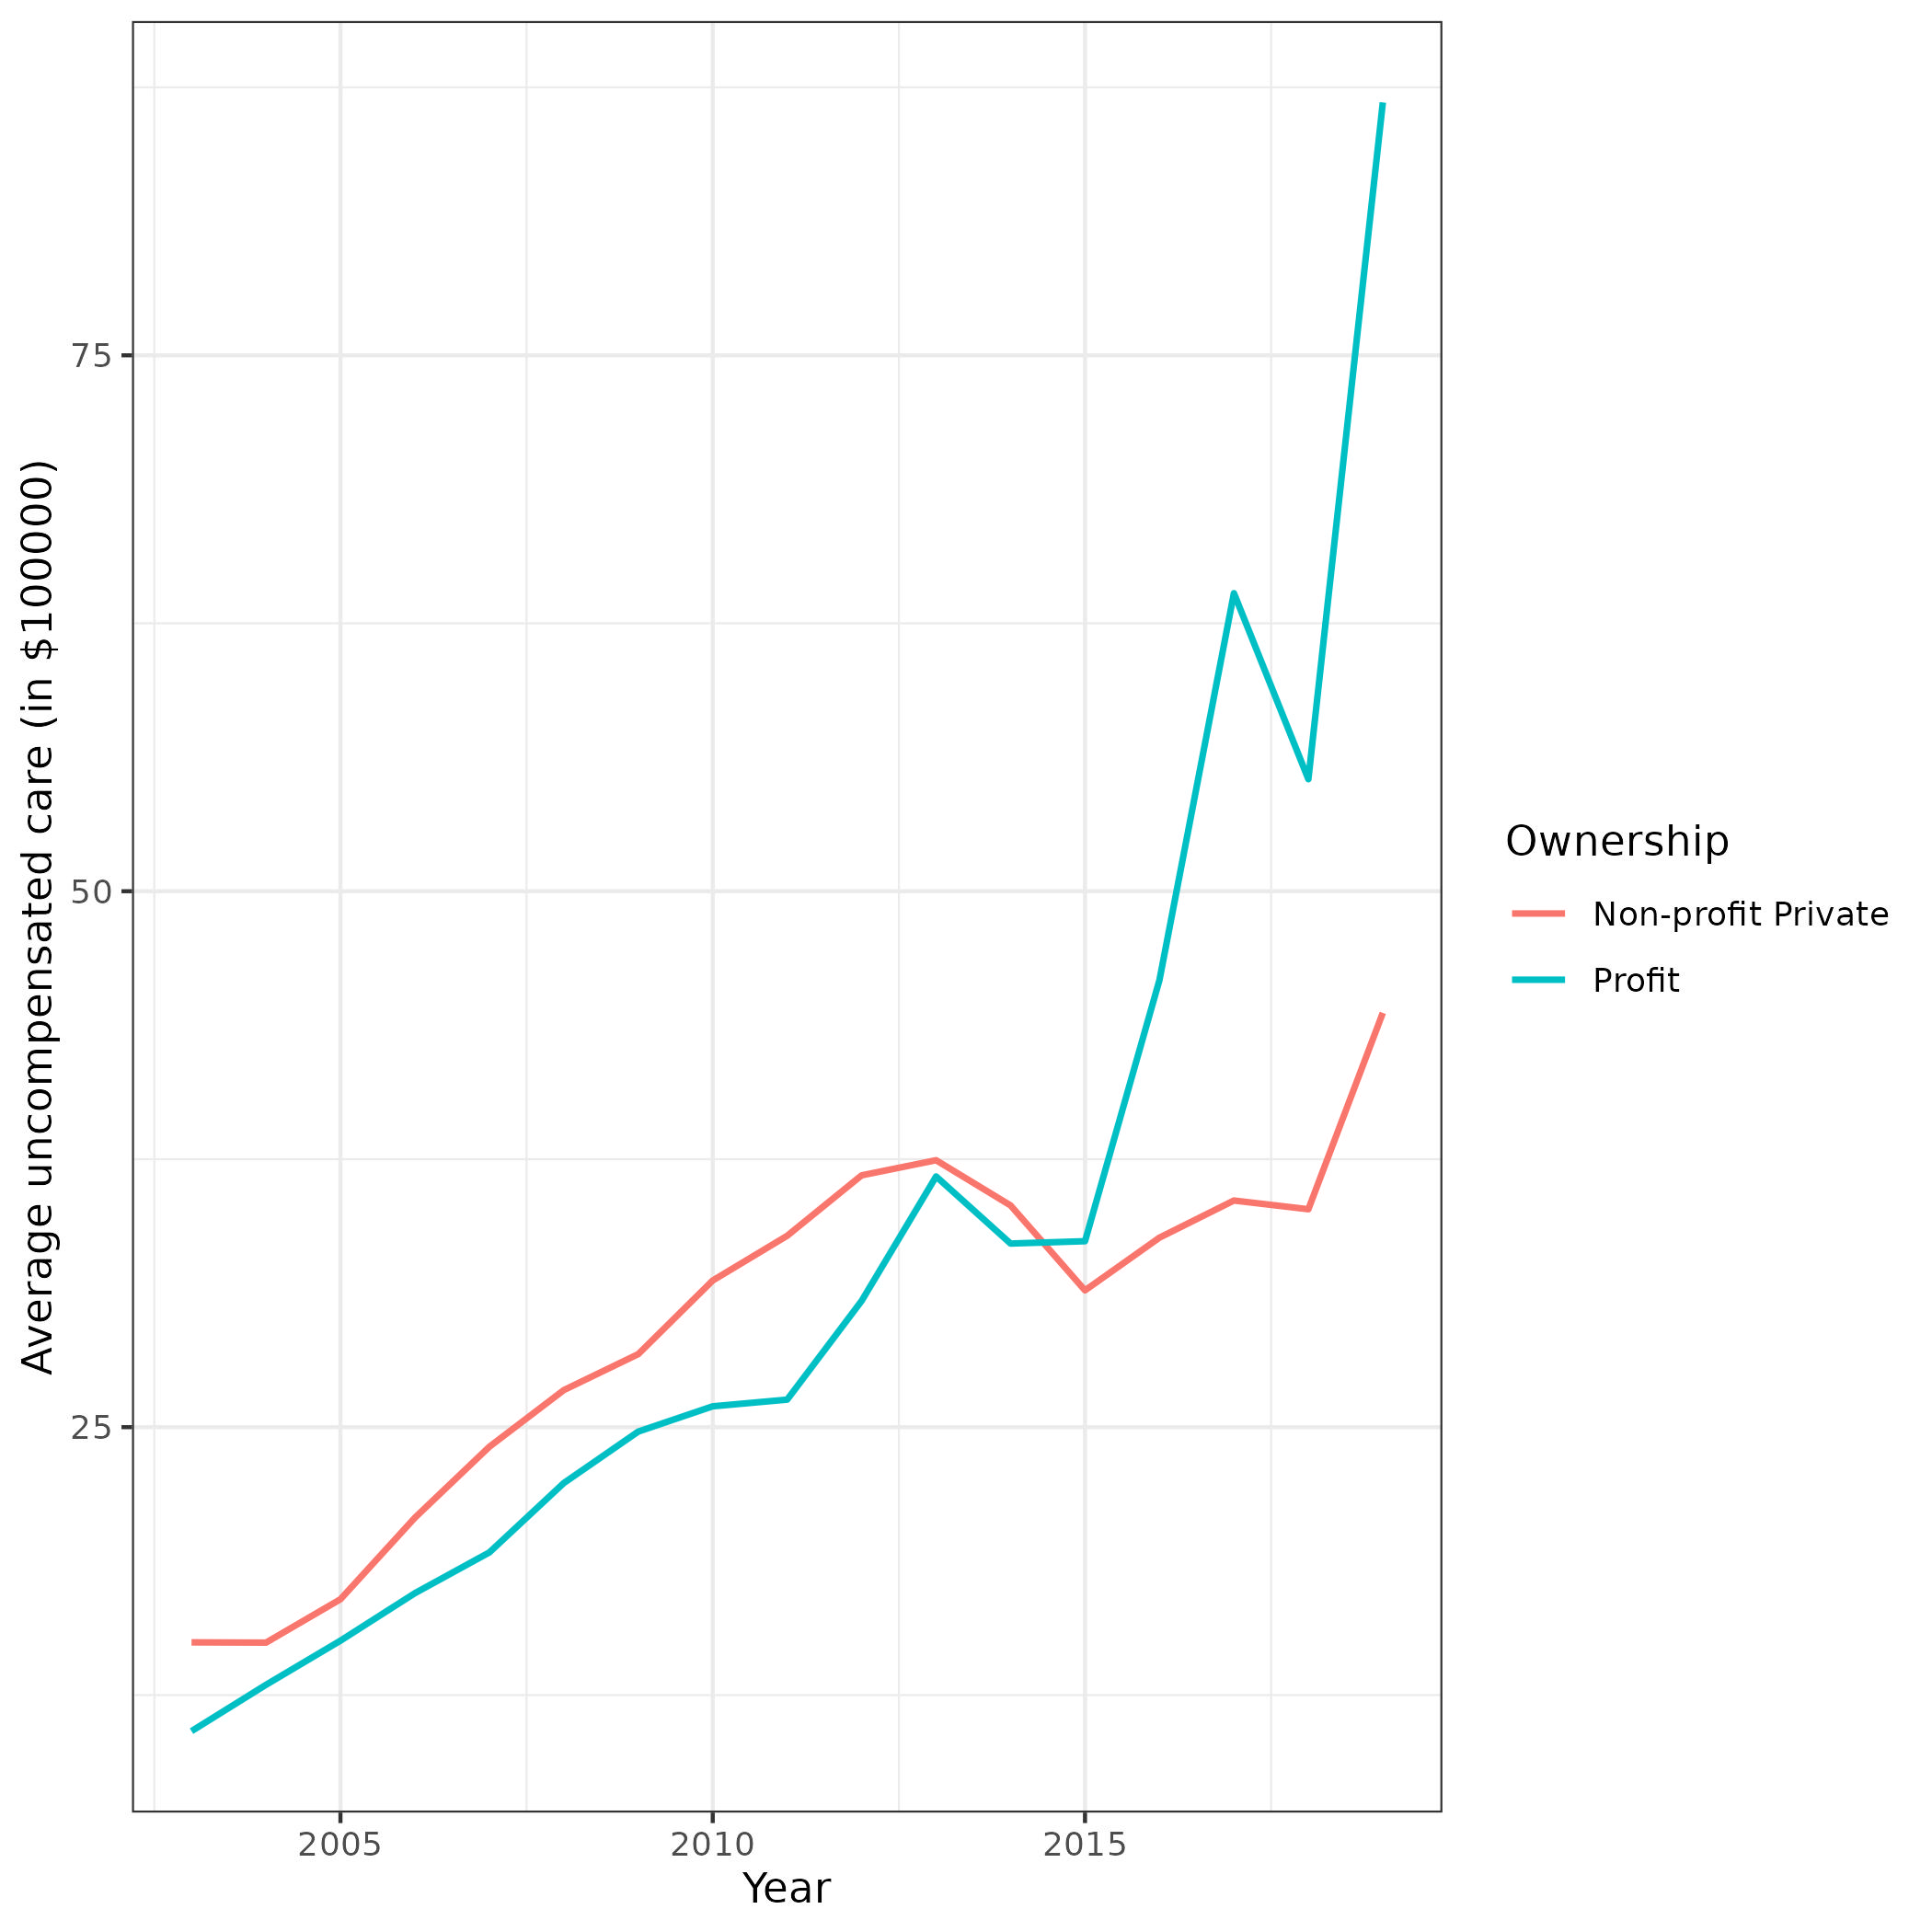
\includegraphics[scale=0.2]{fig_uncompcare.jpg}
			\caption{dd}
		\end{figure}
		The uncompensated care of not-for-profit hospitals increased until 2014, but it seems it stays in the similar level after the Medicaid expansion. On the other hand, the uncompensated care of for-profit hospitals kept increasing.
		
		\item[3.] To estimate the effect of  Medicaid expansion on hospital uncompensated care, I estimate the following two-way fixed effects (TWFE) model.
		\begin{eqnarray}
			y_{it} = \alpha_i + \gamma_t + \delta D_{it} + \epsilon_{it}
		\end{eqnarray}
	    where $D_{it} = 1(E_i \le t)$, $E_i$ is an expansion year, $1(\cdot)$ is an indicator function. $\gamma_t$ denotes time fixed effects, $\alpha_i$ denotes hospital fixed effects, and $y_{it}$ denotes the hospital $i$’s amount of uncompensated care in year $t$.
	    
	    \subfile{../output/tab_twfe}
	    
	    The estimation results are presented in Table 3.  The first column is the result of the estimation using full sample. The coefficient suggests that the exansion of Medicade decreased hospital uncompensated care by 31 million dollars. The second from the fourth column.
	    		
		\item[4.] One can think that the expansion of Medicaid can have a staggered treatment effect. There could be several reasons for the staggered effect. For example, it might takes some times for patients to change their health behavior after the intervention. To investigate the change of the treatment effect over time, I estimate the following event study equation.
		\begin{eqnarray}
			y_{it} = \alpha_i + \gamma_t + \sum_{\tau < -1} D_{it}^{\tau} \delta_{\tau} + \sum_{\tau \ge 0} D_{it}^{\tau} \delta_{\tau} + \epsilon_{it}
		\end{eqnarray}
	    where $D_{it}^{\tau} = 1(t-E_i = \tau)$, $\tau$ denotes years relative to Medicade expansion, so that $\tau = 0$ denotes the year of expansion.
	    
	    \begin{footnotesize}
	    	\begin{table}
	    \subfile{../output/tab_event}
	    \caption{Treatment effect over time}
	    	\end{table}

	    \end{footnotesize}
    
        The estimation results are presented in Table 4. The first column shows that there is a staggered treatment effect. The treatment effect of one year after the intervention was -18.95 and the magnitudes of the effects increase over time.
        The second column shows the subsample estimation results where only states that adopted Medicaid expansion on year 2014 are used as a treatment group. Similarly to the full sample result, the magnitudes of the effects of the expansion keep increasing.
		
		\item[5.] Sun and Abraham (SA) show that the $\delta_{\tau}$ coefficients in equation (2) can be written as a non-convex average of all other group-time specific average treatment effects.
		\begin{eqnarray}
			y_{it} = \alpha_i + \gamma_t + \sum_e \sum_{\tau \neq -1} (D_{it}^{\tau} \times 1(E_i=e)) \delta_{e,\tau} + \epsilon_{it}.
		\end{eqnarray}
		In the following estimation, I investigate whether there are heterogenous treatment effects among the hospitals that adopted the expansion in different years.
		
		\subfile{../output/tab_sunab}
		
		Table 5 shows the estimation result of equation (3). The first column shows the coefficients of the hospitals whose state adopted the exansion in year 2014 and so on. One can see that the treatment effects were larger in the states that adopted Medicaid exapasion later. One possible explanation could be it took some time for the patients in $E=14$ states to acknowledge the policy change, but the patients in $E=16$ states were already aware of the policy change from the other states and were waiting for the policy to be implemented.
		
		\item[6.] Figure 2 shows the event study graph based on the SA estiamtor. It shows the similar results from the event study in aggregate level.
		\begin{figure}
			\centering
			  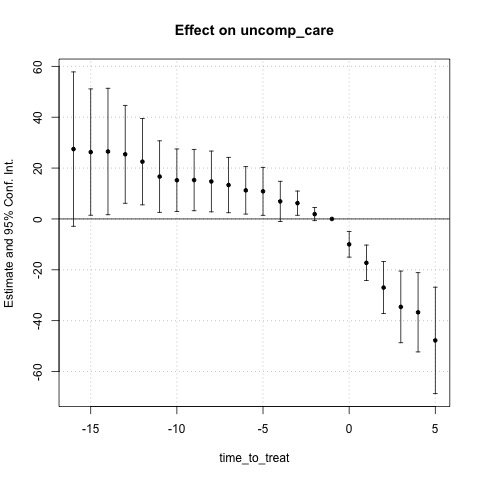
\includegraphics[scale=0.7]{fig_sunab.jpg}
			  \caption{dd}
		\end{figure}
		
		\item[7.] Callaway and Sant'Anna (CS) offer a non-parametric solution that effectively calcuates a set of group-time specific differences. CS also propose aggregations of group-time specific ATT's to form an overall ATT or a time-specific ATT.
		
		Table 6 shows the time-specific aggregated ATT. The treatment effect shows the similar results to the event study.
		
		\begin{tiny}
		\subfile{../output/tab_CS_event}
		\end{tiny}
	
	    \begin{figure}
	    	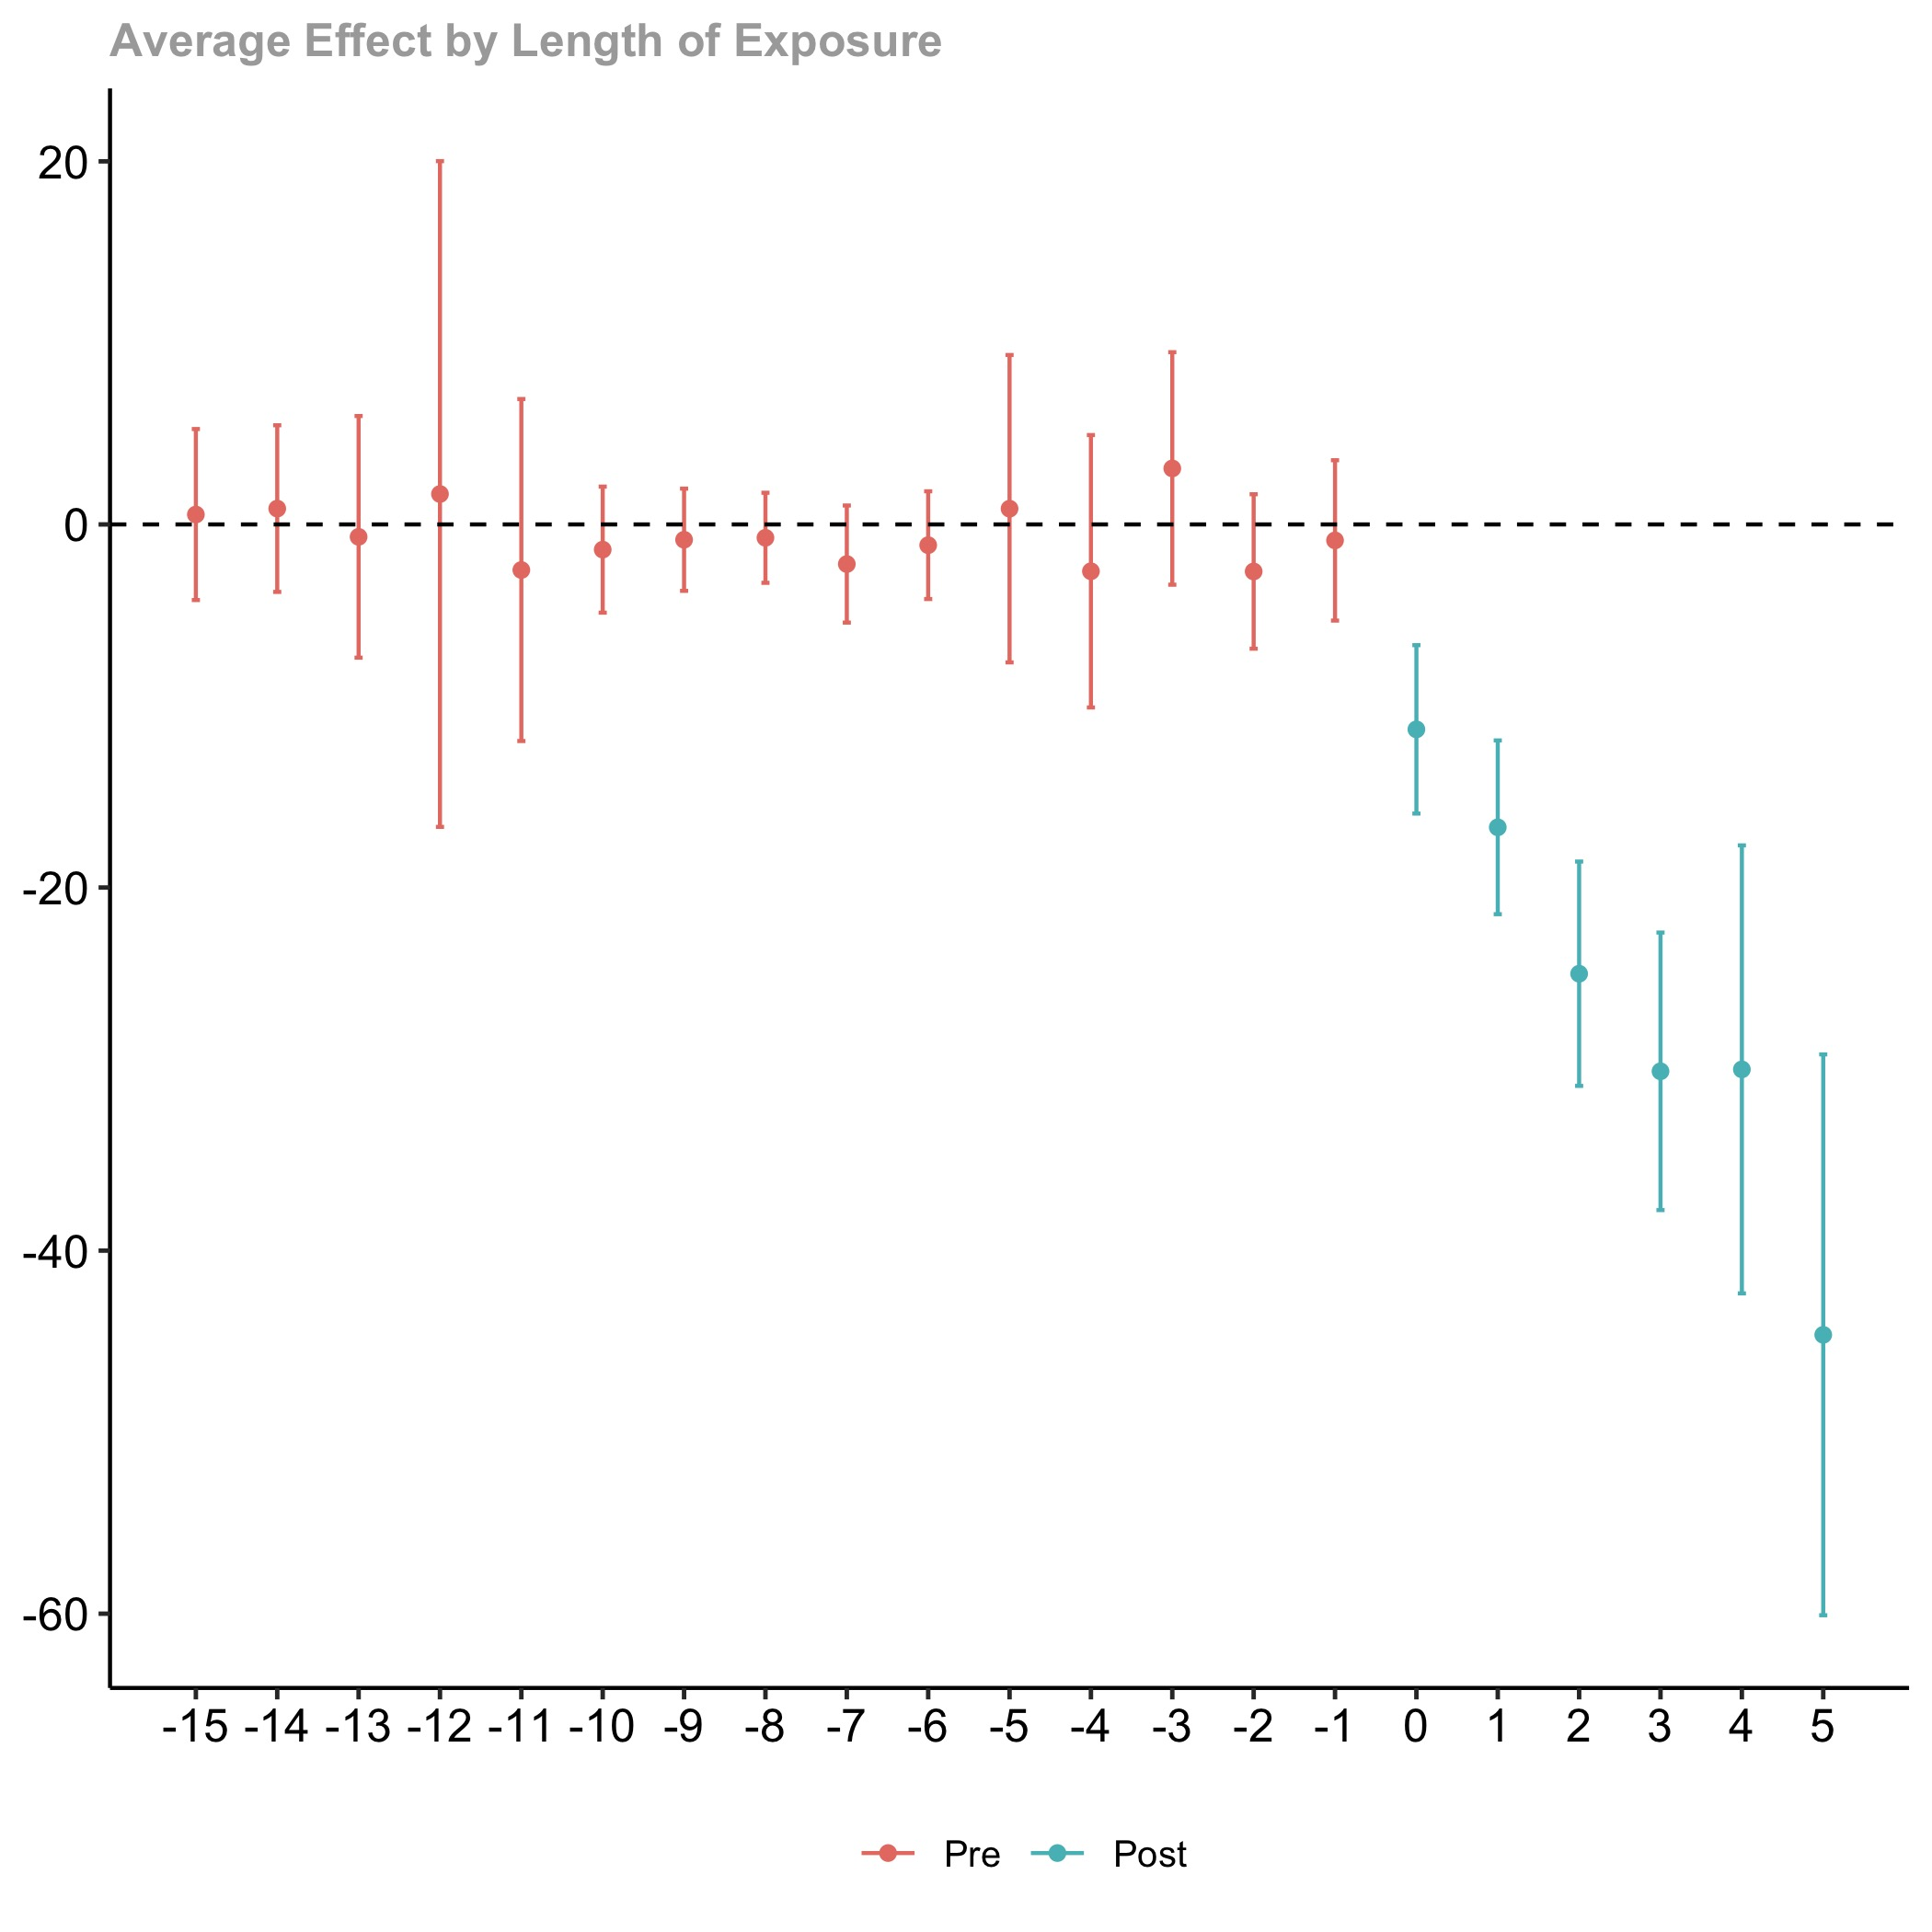
\includegraphics[scale=0.2]{fig_CS_event.jpg}
	    	\caption{Average Effect by Length of Exposure}
	    \end{figure}

		
		\item[8.] The sensitivity results are given in Figure 4.
		
		\begin{figure}
			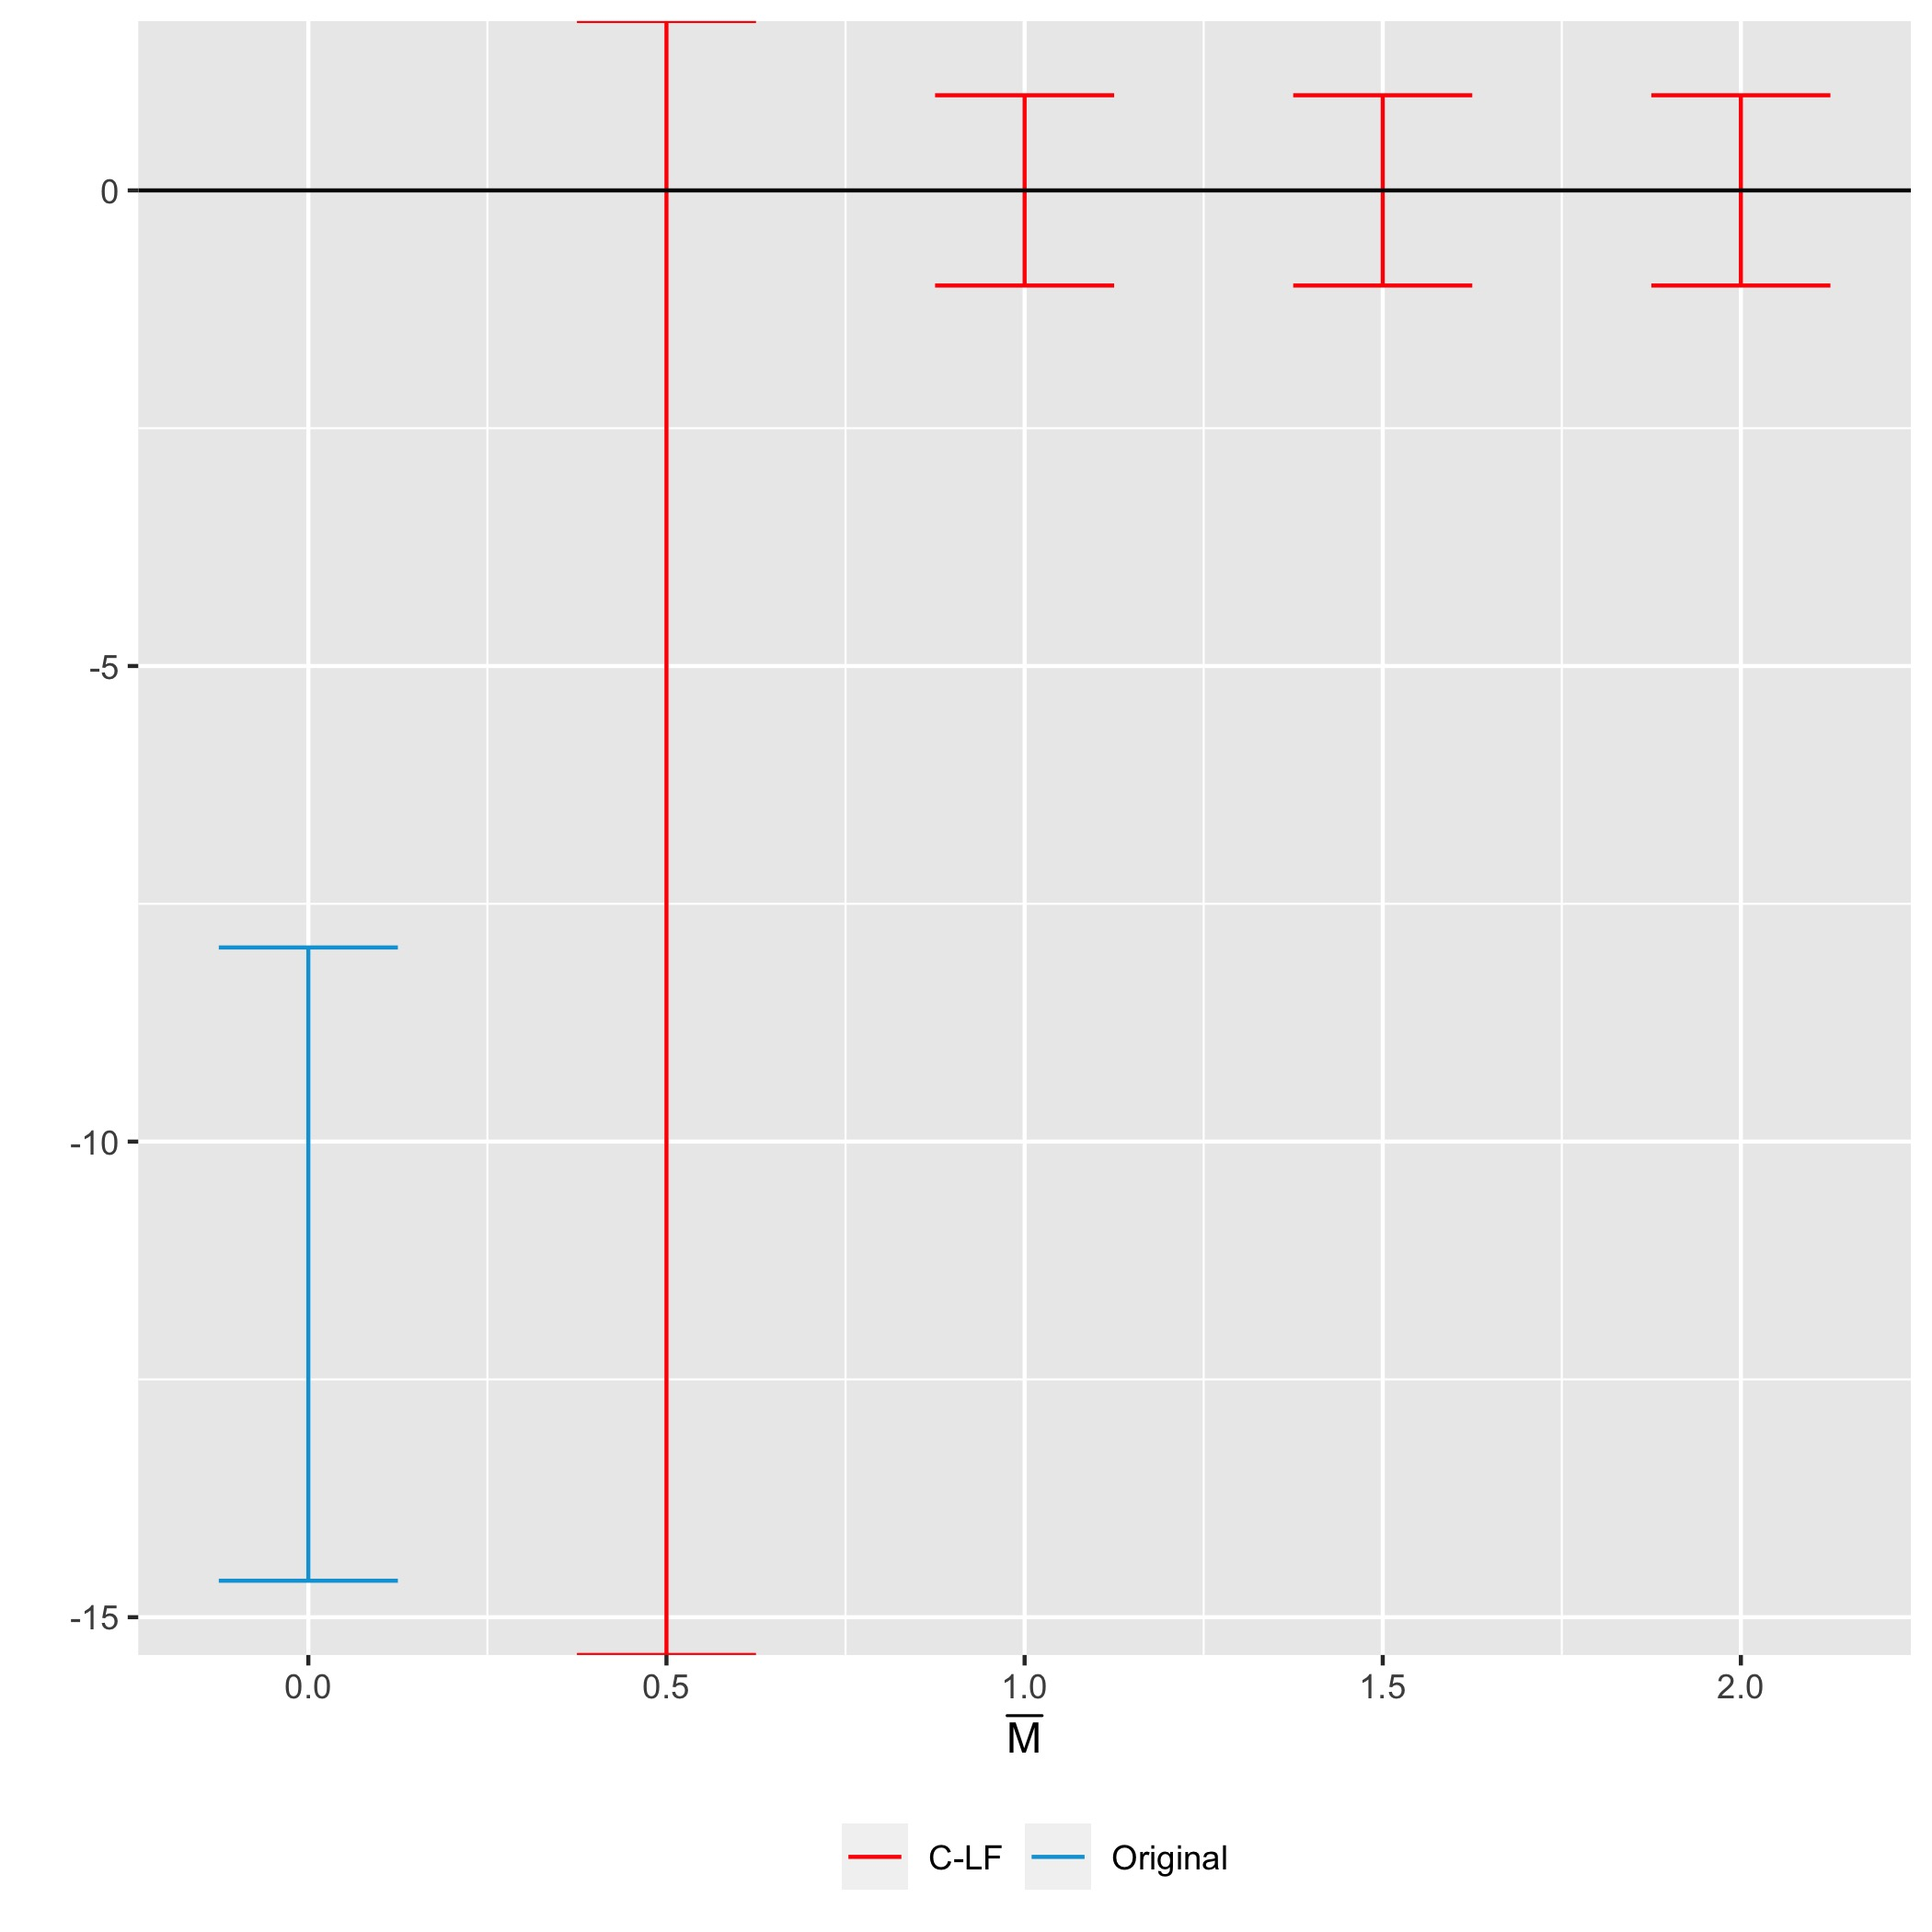
\includegraphics[scale=0.2]{fig_honest.jpg}
			\caption{The sensitivity analysis of  Rambachan and Roth}
		\end{figure}
		
		\item[9.] Overall, the findings were robust to the different specifications and estimations.
		
		\item[10.] I think I could have enjoyed the assignment more if I had started earlier. I did not have enought time to appreciate the ideas of the different estimators. I am very glad that the lecture introduced several cutting-edge estimators in the literature of DD. I will definitely review the estimators in near future.
		
		The most challenging part for me was building up the data, and also producing tables and figures using codes. I need some refinements in my practice, but I think I am on the right direction.
	\end{itemize}
\end{document}